\chapter{Traditional dashboard}
%The dashboard created on PowerBI 
From the KPIs founded in the analysis of the contract we decide to visualize them by creating an off-line dashboard with PowerBi to find other useful information that without visualization could go on the background.

\section{Data cleaning}
Before importing the data, a cleaning of the provided data set must be made to adapt it for the final purpose. 

The main problem is the absence of a field for the dates. For example, data about kilometers run by each member of the consortium were provided as an excel file for each year considered and each file, in turn, was divided in 12 worksheet, one for each operative month. PowerBi needs a reference to join data and to create relationship between different data set, and for this reason, a key about date was created.  

\begin{comment}
\begin{listing}
\inputminted{python}{chapter/code/total_per_month_year.py}
\caption{Code for the merge of the Controllo di gestione}
\label{list:KM_BTS}
\end{listing}
\end{comment}
\section{ER model}
A Entity–relationship model is provided (\ref{fig:ER}) to show the relationships between the different tables.

In detail, the table 'Companies' represents the monthly journeys provided by the Consortium, divided for each companies, from which data about commercial speed and number of rides traveled are extracted for each line. 

The table 'Suppressed rides' is related with 'Companies' through the companies' name. This table gives several information about the events that had as consequence the suppression of a ride; in particular between years 2017 and 2019, it declares the reason for which the ride was suppressed, the line and the company that are associated to that ride. 

'Multi\_Year' is a table related with 'Companies' through line code and it shows introits and costs per kilometer for each line. 

'Flotta' is a table without any relationship and it shows the data about Consortium's fleet for each year between 2018 and 2020 in terms of: emissions and kind of fuel used by each bus, if the bus has air condition, if the bus is equipped for transporting disable people and the age of each bus.


\begin{figure}[h]
    \centering
    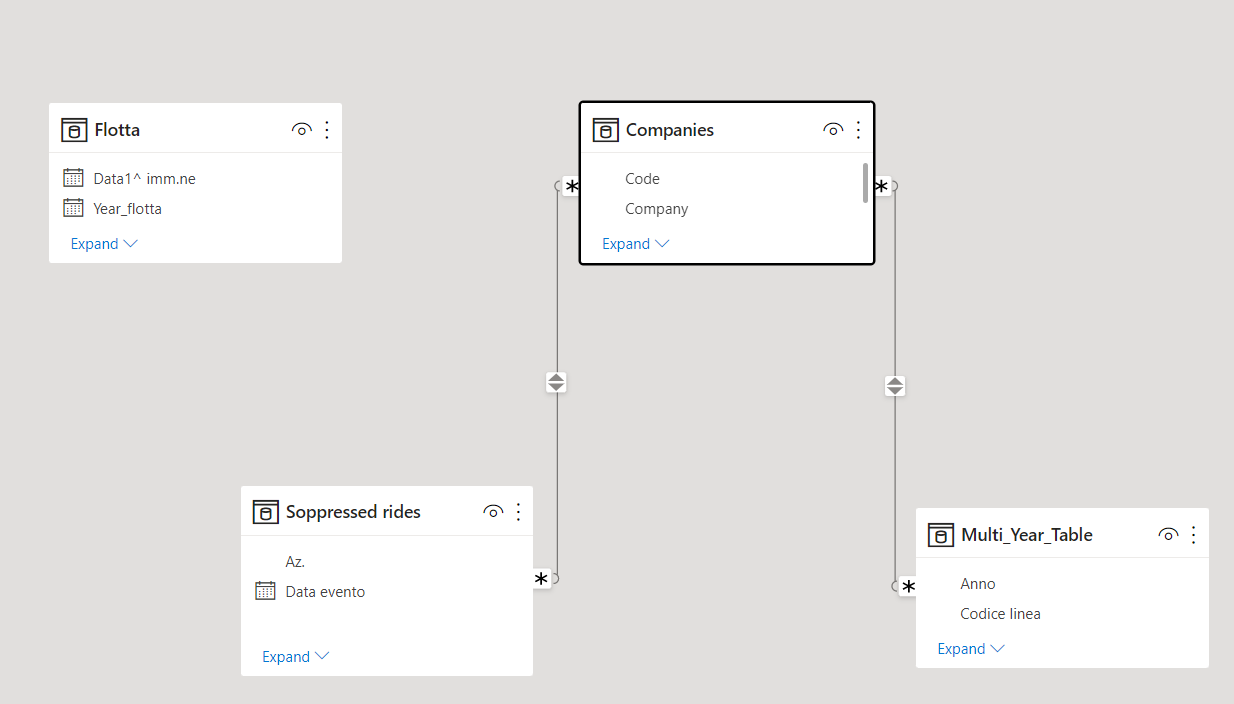
\includegraphics[width=0.9\textwidth]{Images/traditional_dashboard/ER_model.png}
    \caption{ER model of the Dashboard}
    \label{fig:ER}
\end{figure}

